\documentclass[a4paper,12pt]{article} 


\usepackage[T2A]{fontenc}			
\usepackage[utf8]{inputenc}			
\usepackage[english,russian]{babel}	

\usepackage{graphicx, scalerel}    
\usepackage{wrapfig}               
\usepackage[14pt]{extsizes}        
\usepackage[warn]{mathtext}       
\usepackage{indentfirst}      
\usepackage[margin = 25mm]{geometry}
\usepackage[table,xcdraw]{xcolor} 
\usepackage{amsmath,amsfonts,amssymb,amsthm,mathtools}
\usepackage{wasysym}                
\usepackage{upgreek}                
\usepackage{caption}
\usepackage{multirow}
\captionsetup{labelsep=period}
\usepackage[font=small,labelfont=bf]{caption}
\usepackage{gensymb}
\usepackage{icomma}

\usepackage[unicode, pdftex]{hyperref}
\usepackage{tikz}
\usetikzlibrary{positioning}
\usepackage{fancyhdr}
\pagestyle{fancy}
\setlength\fboxsep{3pt} % Отступ рамки \fbox{} от рисунка
\setlength\fboxrule{1pt} % Толщина линий рамки \fbox{}
\usepackage{tocloft}
\newcommand{\tocsection}[1]{\section*{#1} \addcontentsline{toc}{section}{#1}}
\renewcommand{\cftsecleader}{\cftdotfill{\cftdotsep}}




\newcommand{\HRule}{\rule{\linewidth}{0.7mm}} % Defines a new command for the horizontal lines, change thickness here
\begin{document}

\begin{center}
	\large\textbf{Московский Физико-Технический Институт}\\
	\large\textbf{(государственный университет)}
	
	\vfill
	
	
	
	\Large Дополнение к лабораторной работе 5.2.1
	%----------------------------------------------------------------------------------------
	%	TITLE SECTION
	%----------------------------------------------------------------------------------------

	
	\ \\
	\textbf{\large Автор:} \\	
	\large Овсянников Михаил Б01-008\\
	\vfill
	\hspace*{-0.8 cm}
\includegraphics[width=100 pt]{./Include/frkt_logo.pdf}\\
	\large Долгопрудный, 2022
\end{center}

\thispagestyle{empty}

\newpage
\setcounter{page}{2}
\fancyfoot[c]{\thepage}
\fancyhead[L] {Дополнение к лабораторной работе 5.2.1}
\fancyhead[R] {Опыт Франка–Герца}


В работе 5.2.1 воспроизвелся опыт Франка-Герца, подтверждающий наличие дискретных уровней возбуждения атомов. В частности, исследовался инертный газ -- гелий. По статическому методу было определено значение энергии возбуждения первого уровня атома гелия: $E = (21,6 \pm 0,3)$ эВ. Однако оно было определено по расстояниям между максимумами (минимумами) на ВАХ, которые хоть и были выражены, но недостаточно. В данном дополнении предлагается улучшить методику.

Представим общий коллекторный ток $I_\text{к}$ в виде вот такой вот суммы:

\begin{equation*}
	I_\text{к} = I_0 + I_\sim,
\end{equation*}
где $I_0$ -- это ток, предсказанный классической теорией, то есть сначала возрастающий по закону $3/2$, а затем выходящий на плато -- насыщение; а $I_\sim$ -- это ток, который и дает осцилляцию истинному значению коллекторного тока.

Сделав это, мы сможем наблюдать более выраженные максимумы и минимумы на зависимости $I_\sim (V_a)$, поэтому будет легче посчитать $\Delta V$, и, что еще лучше, это будет гораздо точнее! 

Чтобы найти зависимость $I_0(V_a)$, пройдемся по <<средним>> точкам графиков для каждого из значений задерживающего напряжения. После этого аппроксимируем полученные точки кривой насыщения.

Чтобы найти зависимость $I_\sim (V_a)$, просто вычтем из $I_\text{к}$ значение $I_0$:
\begin{equation*}
	I_\sim (V_a) = I_\text{к}(V_a) - I_0 (V_a)
\end{equation*}

Не будем здесь описывать всю процедуру с технической стороны, а сразу приведем полученные графики для $I_\sim (V_a)$ при различных значениях задерживающего напряжения.


\begin{figure}[h!]
	\centering
	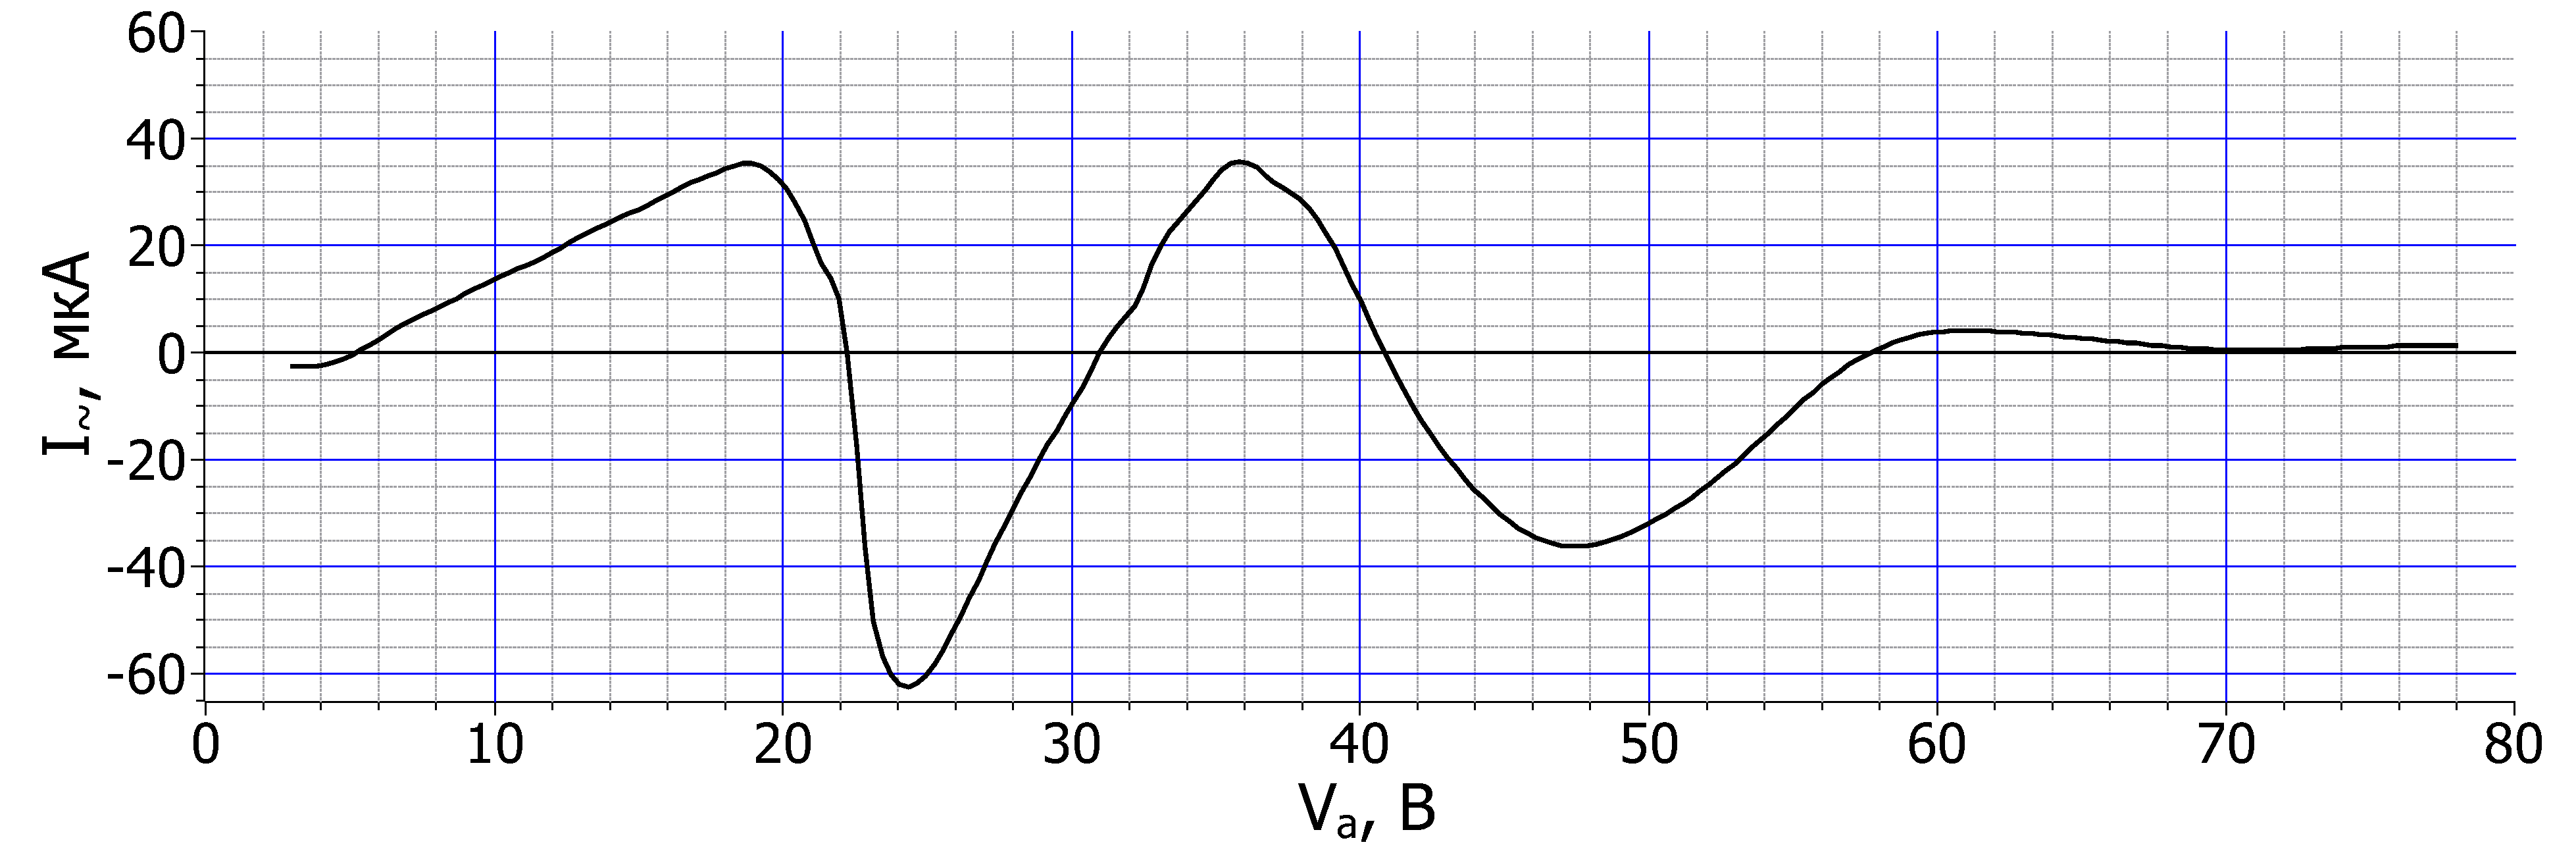
\includegraphics[width=\linewidth]{./Pictures/I_tilde(V)_4V.pdf}
	\caption{$I_\sim (V_a)$ при задерживающем напряжении 4 В}
\end{figure}

По графику получаем:
\begin{equation*}
	\Delta V = (21,79 \pm 0,07) \text{ В}
\end{equation*}


\newpage
\begin{figure}[h!]
	\centering
	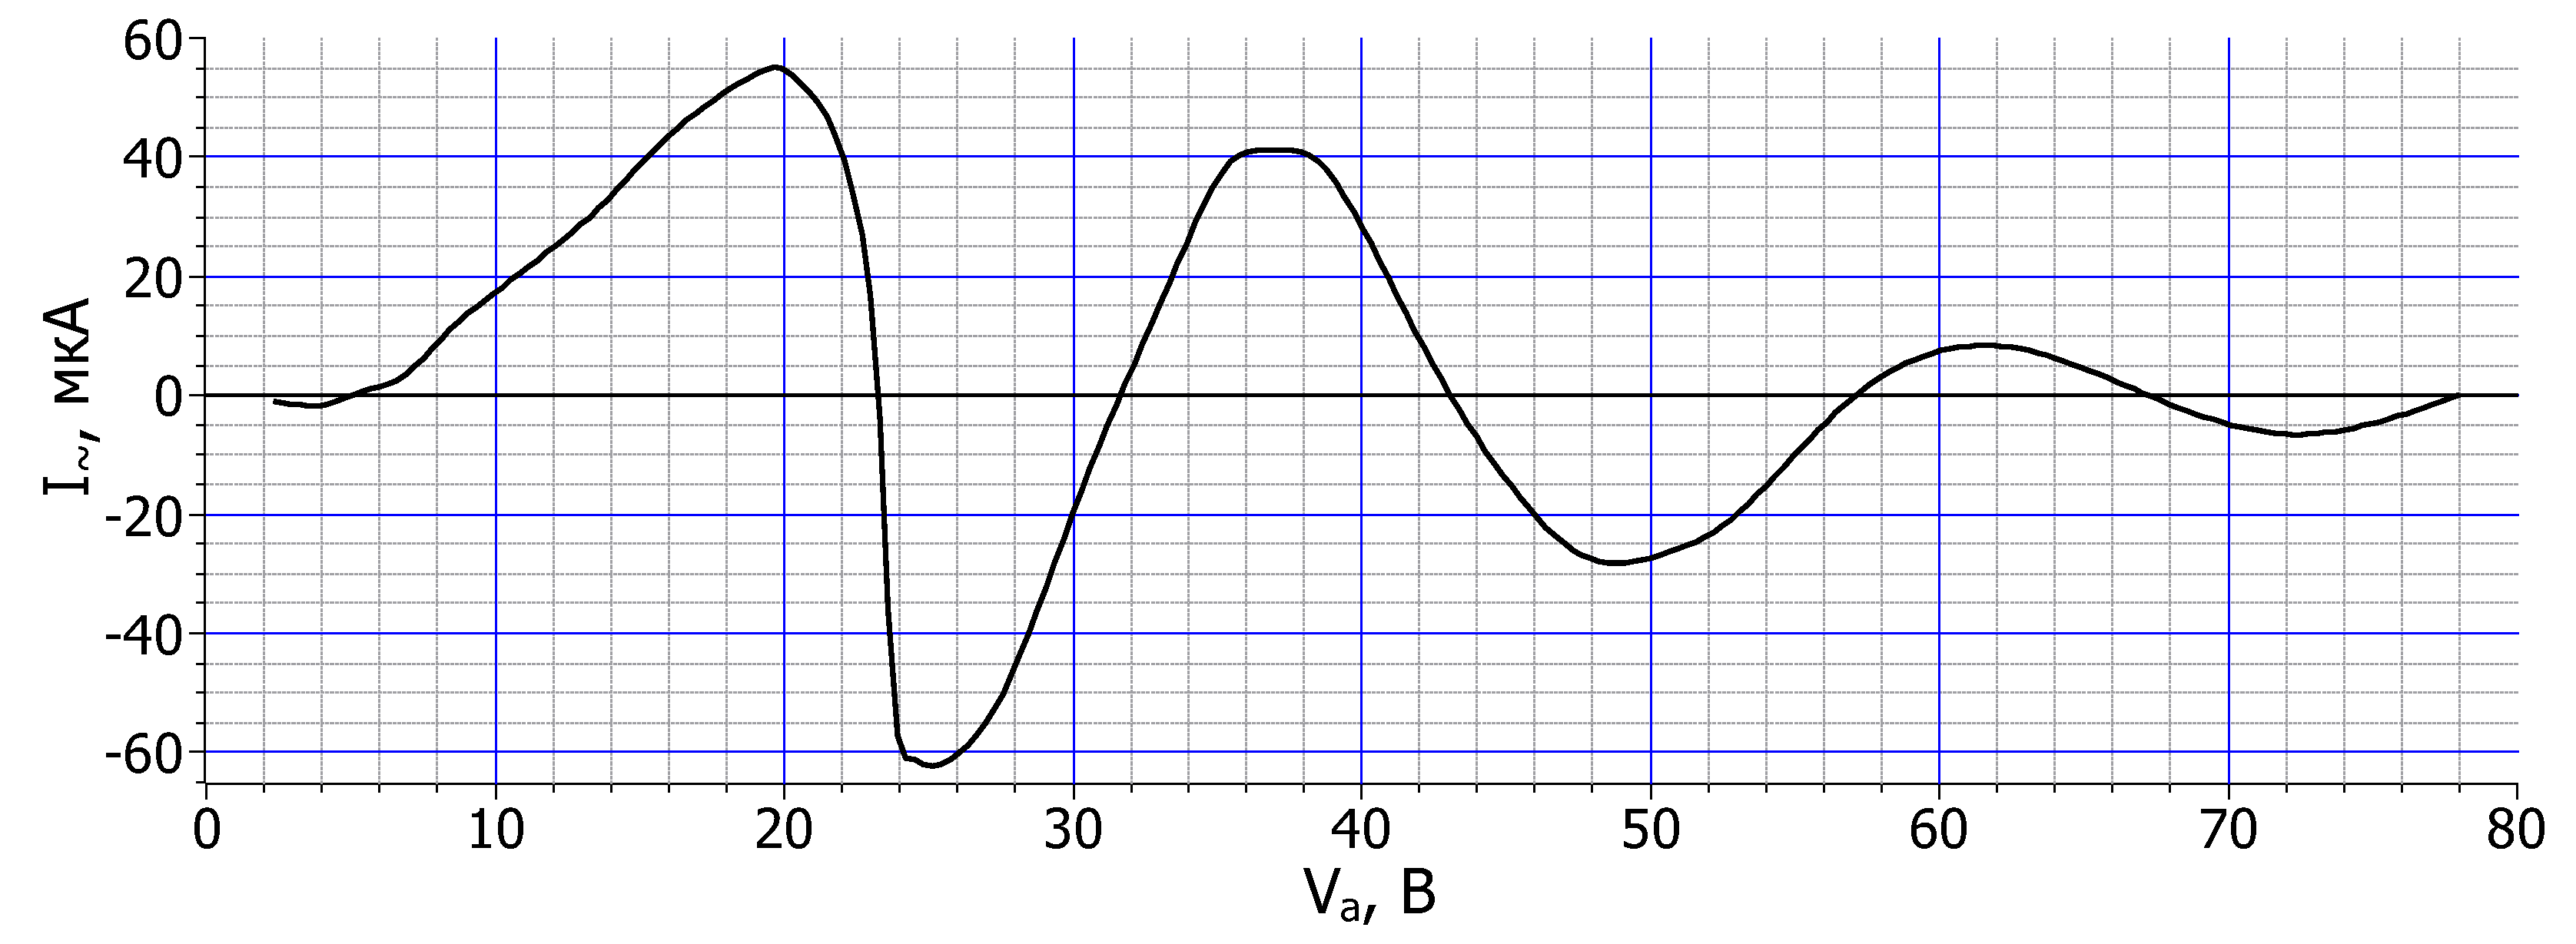
\includegraphics[width=\linewidth]{./Pictures/I_tilde(V)_6V.pdf}
	\caption{$I_\sim (V_a)$ при задерживающем напряжении 6 В}
\end{figure}

По этому графику получаем:
\begin{equation*}
	\Delta V = (21,71 \pm 0,06) \text{ В}
\end{equation*}


\begin{figure}[h!]
	\centering
	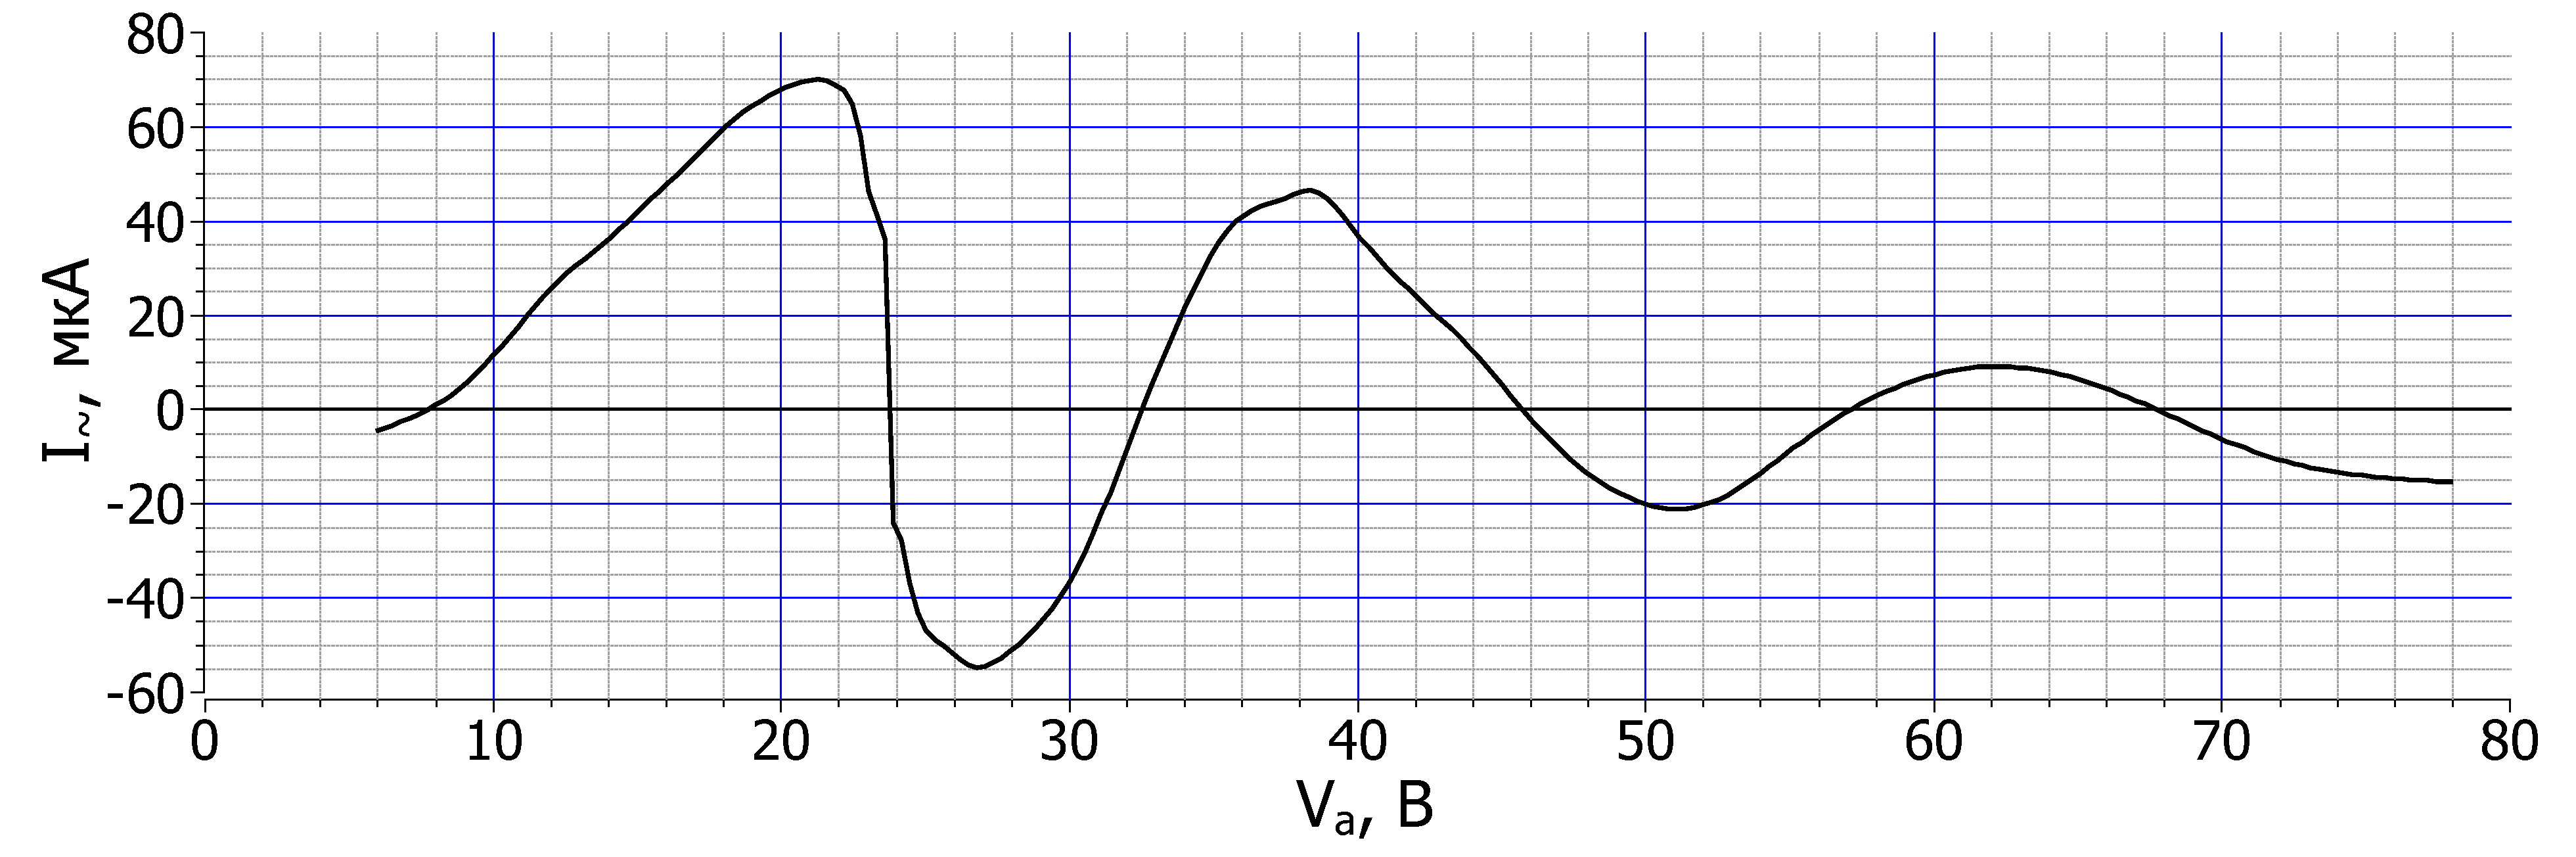
\includegraphics[width=\linewidth]{./Pictures/I_tilde(V)_8V.pdf}
	\caption{$I_\sim (V_a)$ при задерживающем напряжении 8 В}
\end{figure}

А здесь выходит:
\begin{equation*}
	\Delta V = (21,7 \pm 0,1) \text{ В}
\end{equation*}

В среднем
\begin{equation*}
	\boxed{\Delta V^\Sigma = (21,7 \pm 0,2) \text{ В}}
\end{equation*}

Как видим, точность действительно увеличилась, хоть и не на порядки. И даже получившийся интервал почти полностью лежит в интервале, полученном ранее.

\end{document}
